\begin{filecontents}{references.bib}
@article{kingma2014adam,
  title={Adam: A Method for Stochastic Optimization},
  author={Kingma, Diederik P and Ba, Jimmy},
  journal={arXiv preprint arXiv:1412.6980},
  year={2014}
}

@inproceedings{he2016deep,
  title={Deep Residual Learning for Image Recognition},
  author={He, Kaiming and Zhang, Xiangyu and Ren, Shaoqing and Sun, Jian},
  booktitle={Proceedings of the IEEE Conference on Computer Vision and Pattern Recognition (CVPR)},
  pages={770--778},
  year={2016}
}
\end{filecontents}

\documentclass{article}

\usepackage[table]{xcolor}
\usepackage{graphicx}
\usepackage{natbib}
\usepackage{url}

% ICLR 2025 Workshop style is assumed to be provided; below is a placeholder.
\usepackage[margin=1in]{geometry}

\graphicspath{{figures/}}

\title{Troublesome Model Inconsistencies in Real-World Deployment}
\author{Anonymous Submission}
\date{}

\begin{document}

\maketitle

\begin{abstract}
Deep learning systems often present unexpected pitfalls when moved from controlled research environs to real-world settings. We investigate subtle inconsistencies in training behaviors, revealing partially negative or inconclusive results. Our findings can guide better deployment strategies and highlight the need for caution when relying on standard training heuristics.
\end{abstract}

\section{Introduction}
Real-world deployment of deep neural networks frequently exposes brittleness and setbacks not obvious in controlled benchmarks. In this paper, we analyze inconsistencies observed when fine-tuning with standard optimizers \citep{kingma2014adam} and network backbones \citep{he2016deep}, focusing on problems such as training collapse in certain conditions. Although we attempted multiple adjustments (e.g., modest hyperparameter tuning, alternative layer initializations), many improvements were incremental or inconclusive. These challenges merit attention because of deployment safety and reliability implications.

\section{Related Work}
Other researchers have identified phenomena such as vanishing gradients and over-fitting under domain shifts. Studies have explored specific failure cases and partial mitigations but rely on strong assumptions about data distribution. While there exist methods to improve stability, their real-world performance may still be fragile. This work differs by offering a comprehensive view of pitfalls in multiple training regimes, providing guidance on how factors like data preprocessing can fail silently.

\section{Method / Problem Discussion}
Our investigation centers on a simple classification pipeline. We first pre-train on a large dataset before fine-tuning on a smaller, possibly mismatched target domain. Standard procedures can yield deceptively promising validation metrics until encountering atypical data. Much of our analysis was through repeated runs across varying seeds and slight model variations. We highlight scenarios where basic design choices disrupted expected behaviors.

\section{Experiments}
We performed initial experimentation with a ResNet-50 backbone \citep{he2016deep} using the Adam optimizer \citep{kingma2014adam}. Figures~\ref{fig:baseline_pretrain} and~\ref{fig:baseline_finetune} illustrate the training curves for baseline pre-training and fine-tuning, respectively. Some runs converged predictably, whereas others showed sharp drop-offs with marginally altered augmentations, culminating in inconsistent final accuracies. Attempts to remedy these drops via small hyperparameter tweaks yielded negligible benefit and occasionally worsened divergence.

\begin{figure}[t]
\centering
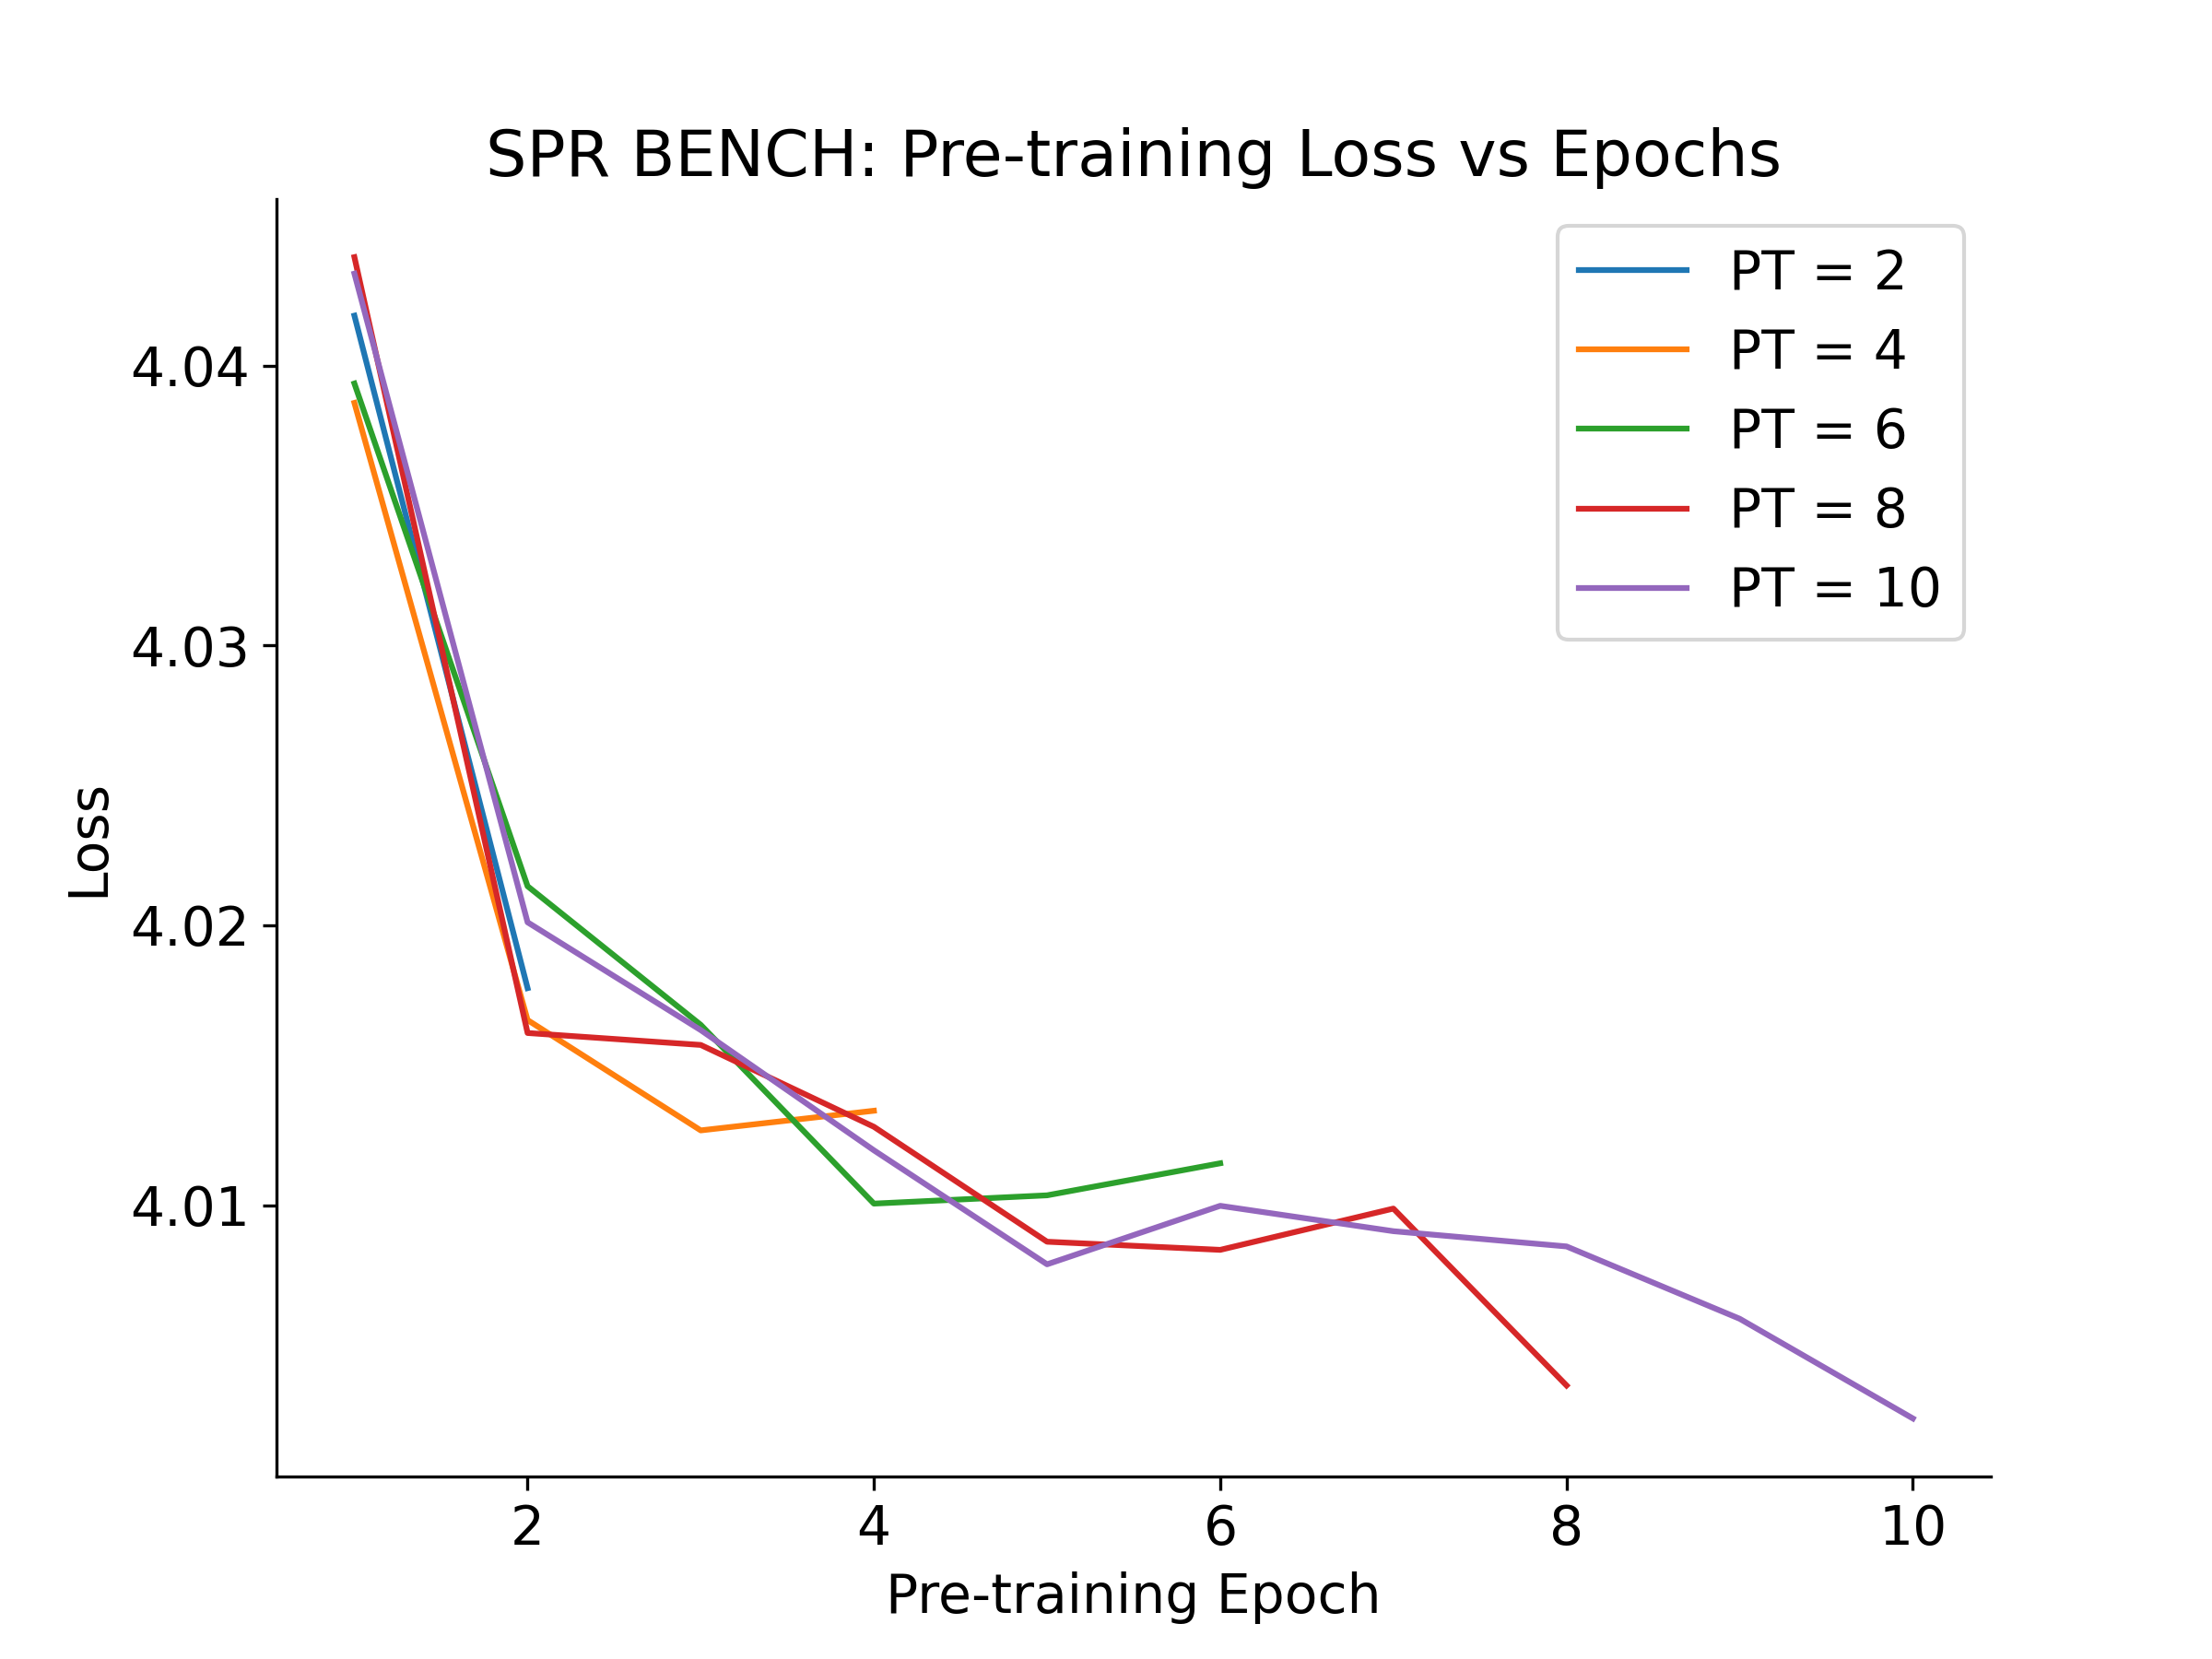
\includegraphics[width=0.45\textwidth]{baseline_pretrain_loss.png}
\caption{Pre-training loss. Some runs remain stable, while others show erratic dips with minor changes.}
\label{fig:baseline_pretrain}
\end{figure}

\begin{figure}[t]
\centering
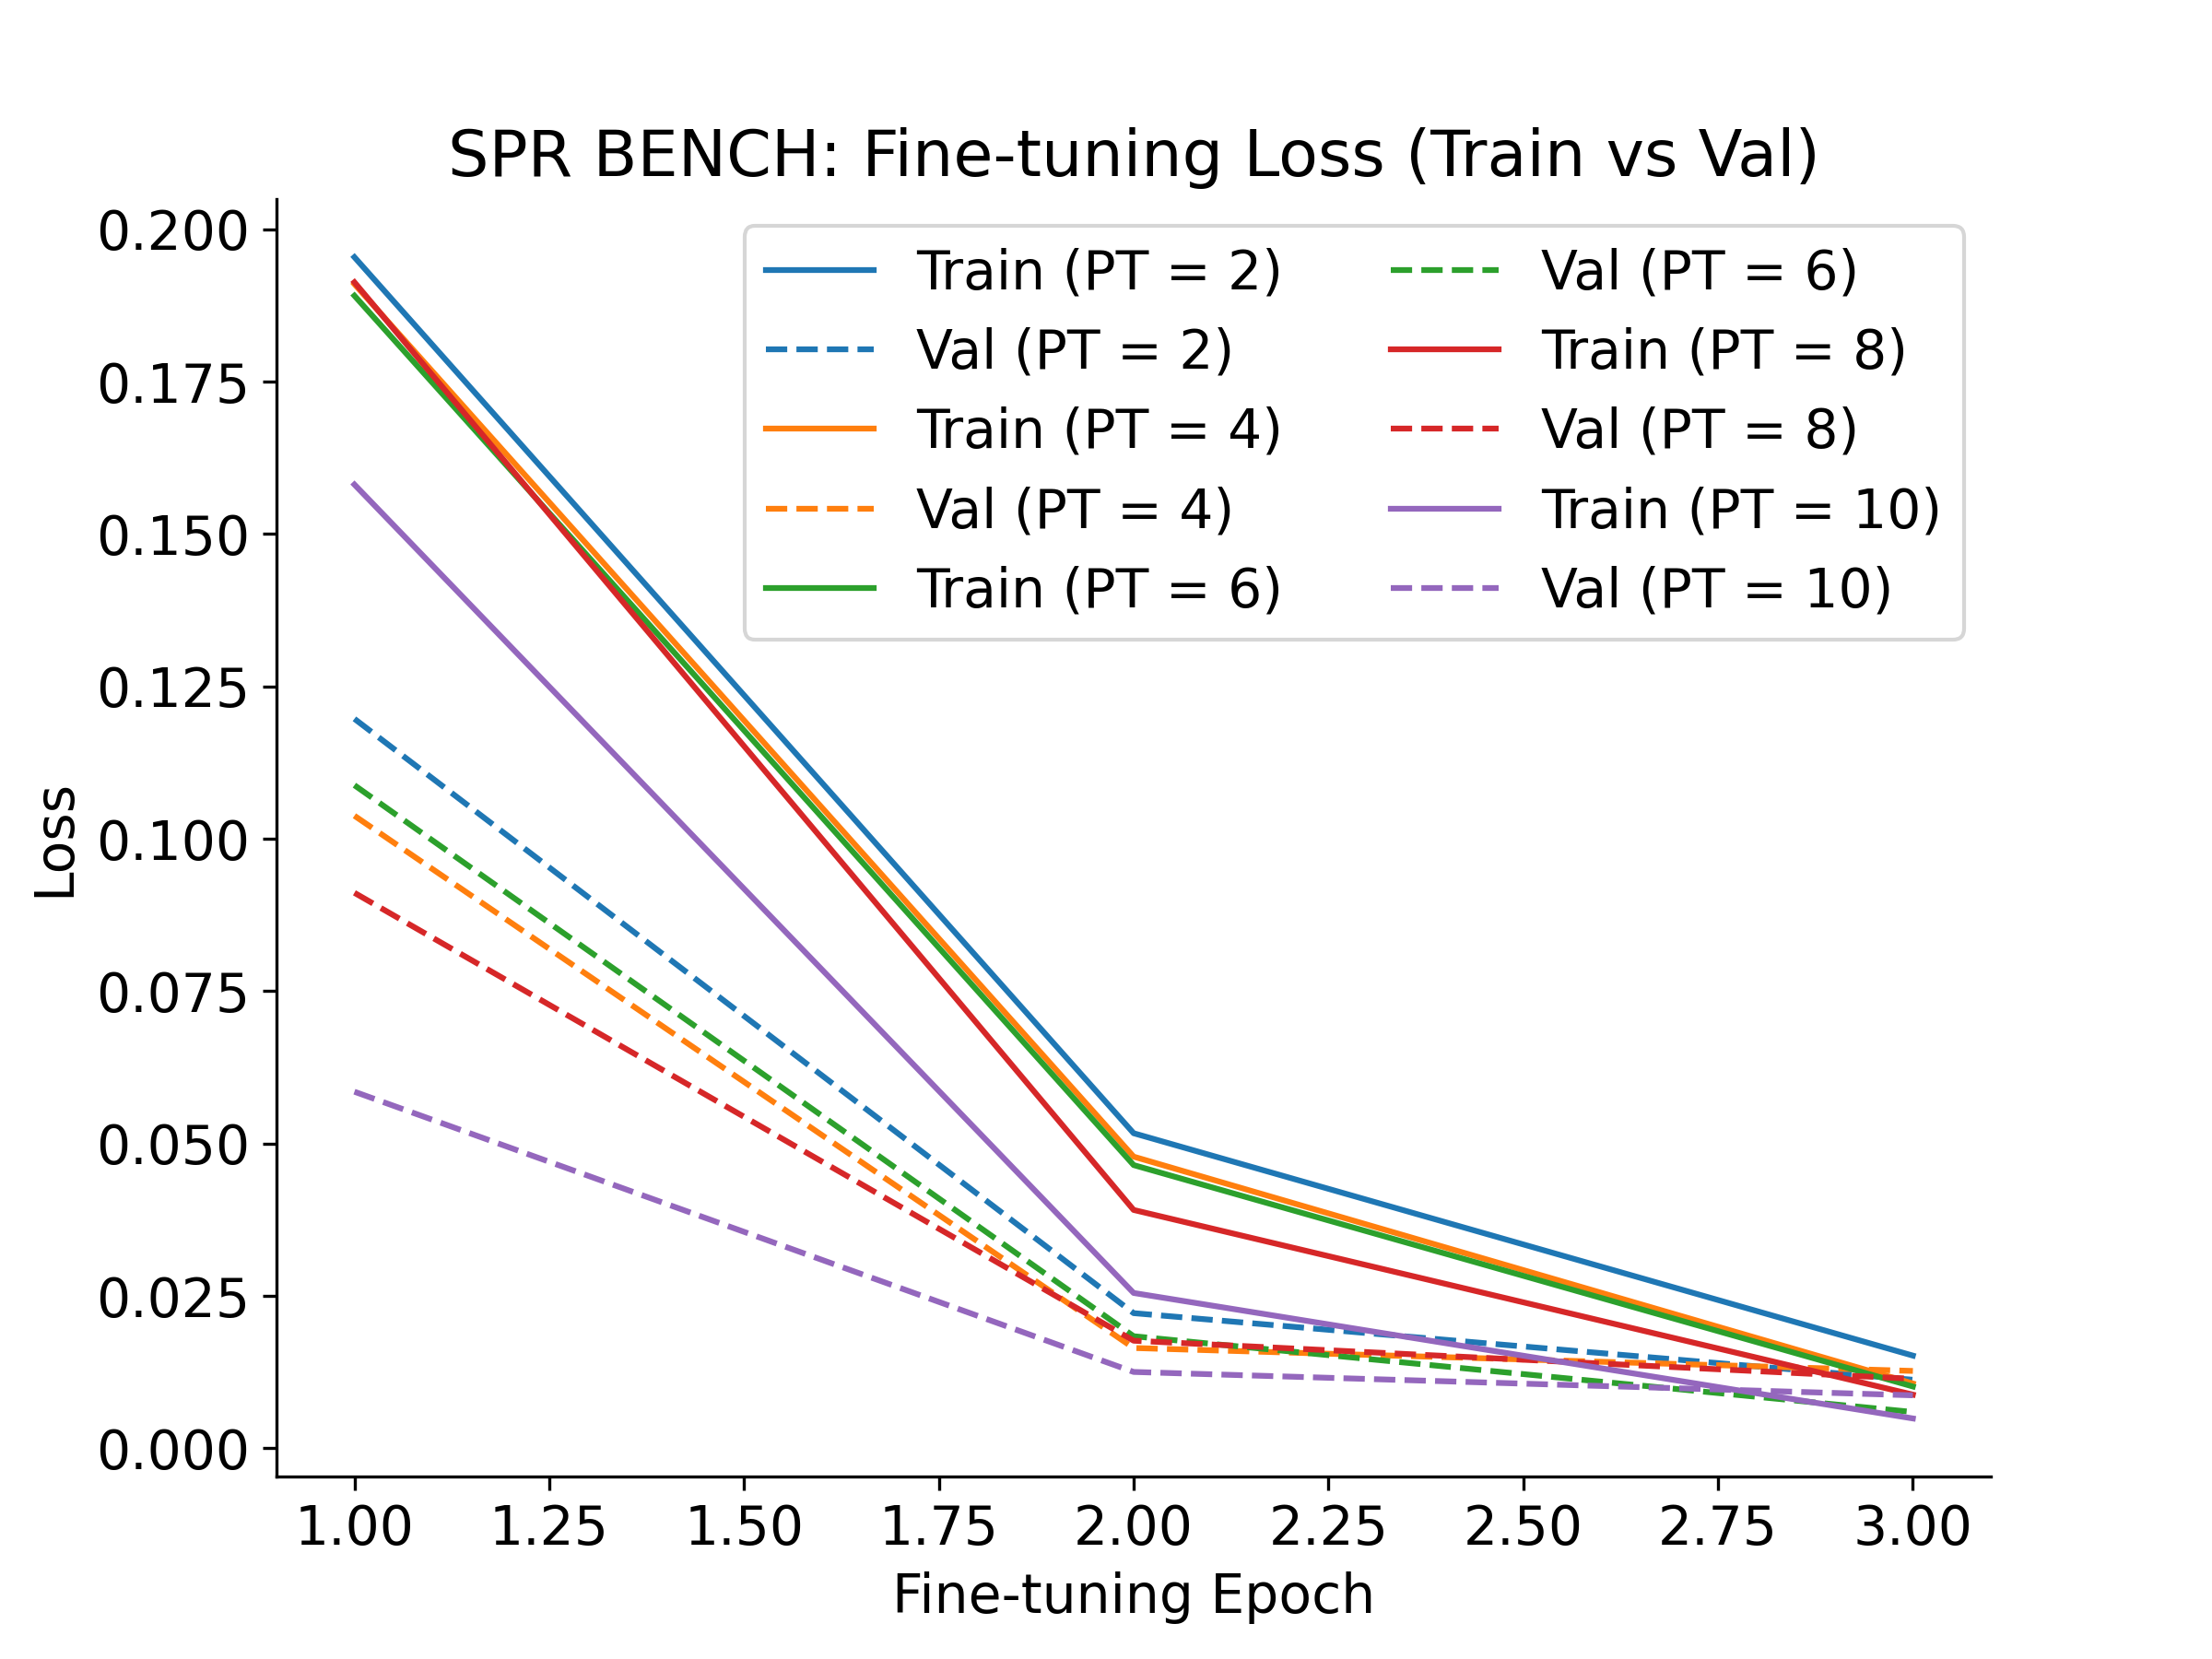
\includegraphics[width=0.45\textwidth]{baseline_finetune_loss.png}
\caption{Fine-tuning loss. Sudden fluctuations appear in apparently similar setups.}
\label{fig:baseline_finetune}
\end{figure}

Figure~\ref{fig:research_pretrain_loss} (Appendix) displays a similar pattern in a different configuration, reinforcing the complexity of identifying consistent outcomes.

\section{Conclusion}
We explored deep learning inconsistencies emerging under routine model deployment steps. Though partial fixes exist, they did not uniformly resolve the issues. Future work could focus on rigorous stress testing across diverse data scenarios. By emphasizing reproducibility and transparent disclosure of negative results, the community can develop more robust network design and training principles.

\clearpage
\bibliography{references}
\bibliographystyle{plainnat}

\appendix
\section{Supplementary Material}
Here we present additional plots and hyperparameter details. Figure~\ref{fig:research_pretrain_loss} shows a representative pre-training attempt with slight variations in seed initialization.

\begin{figure}[h]
\centering
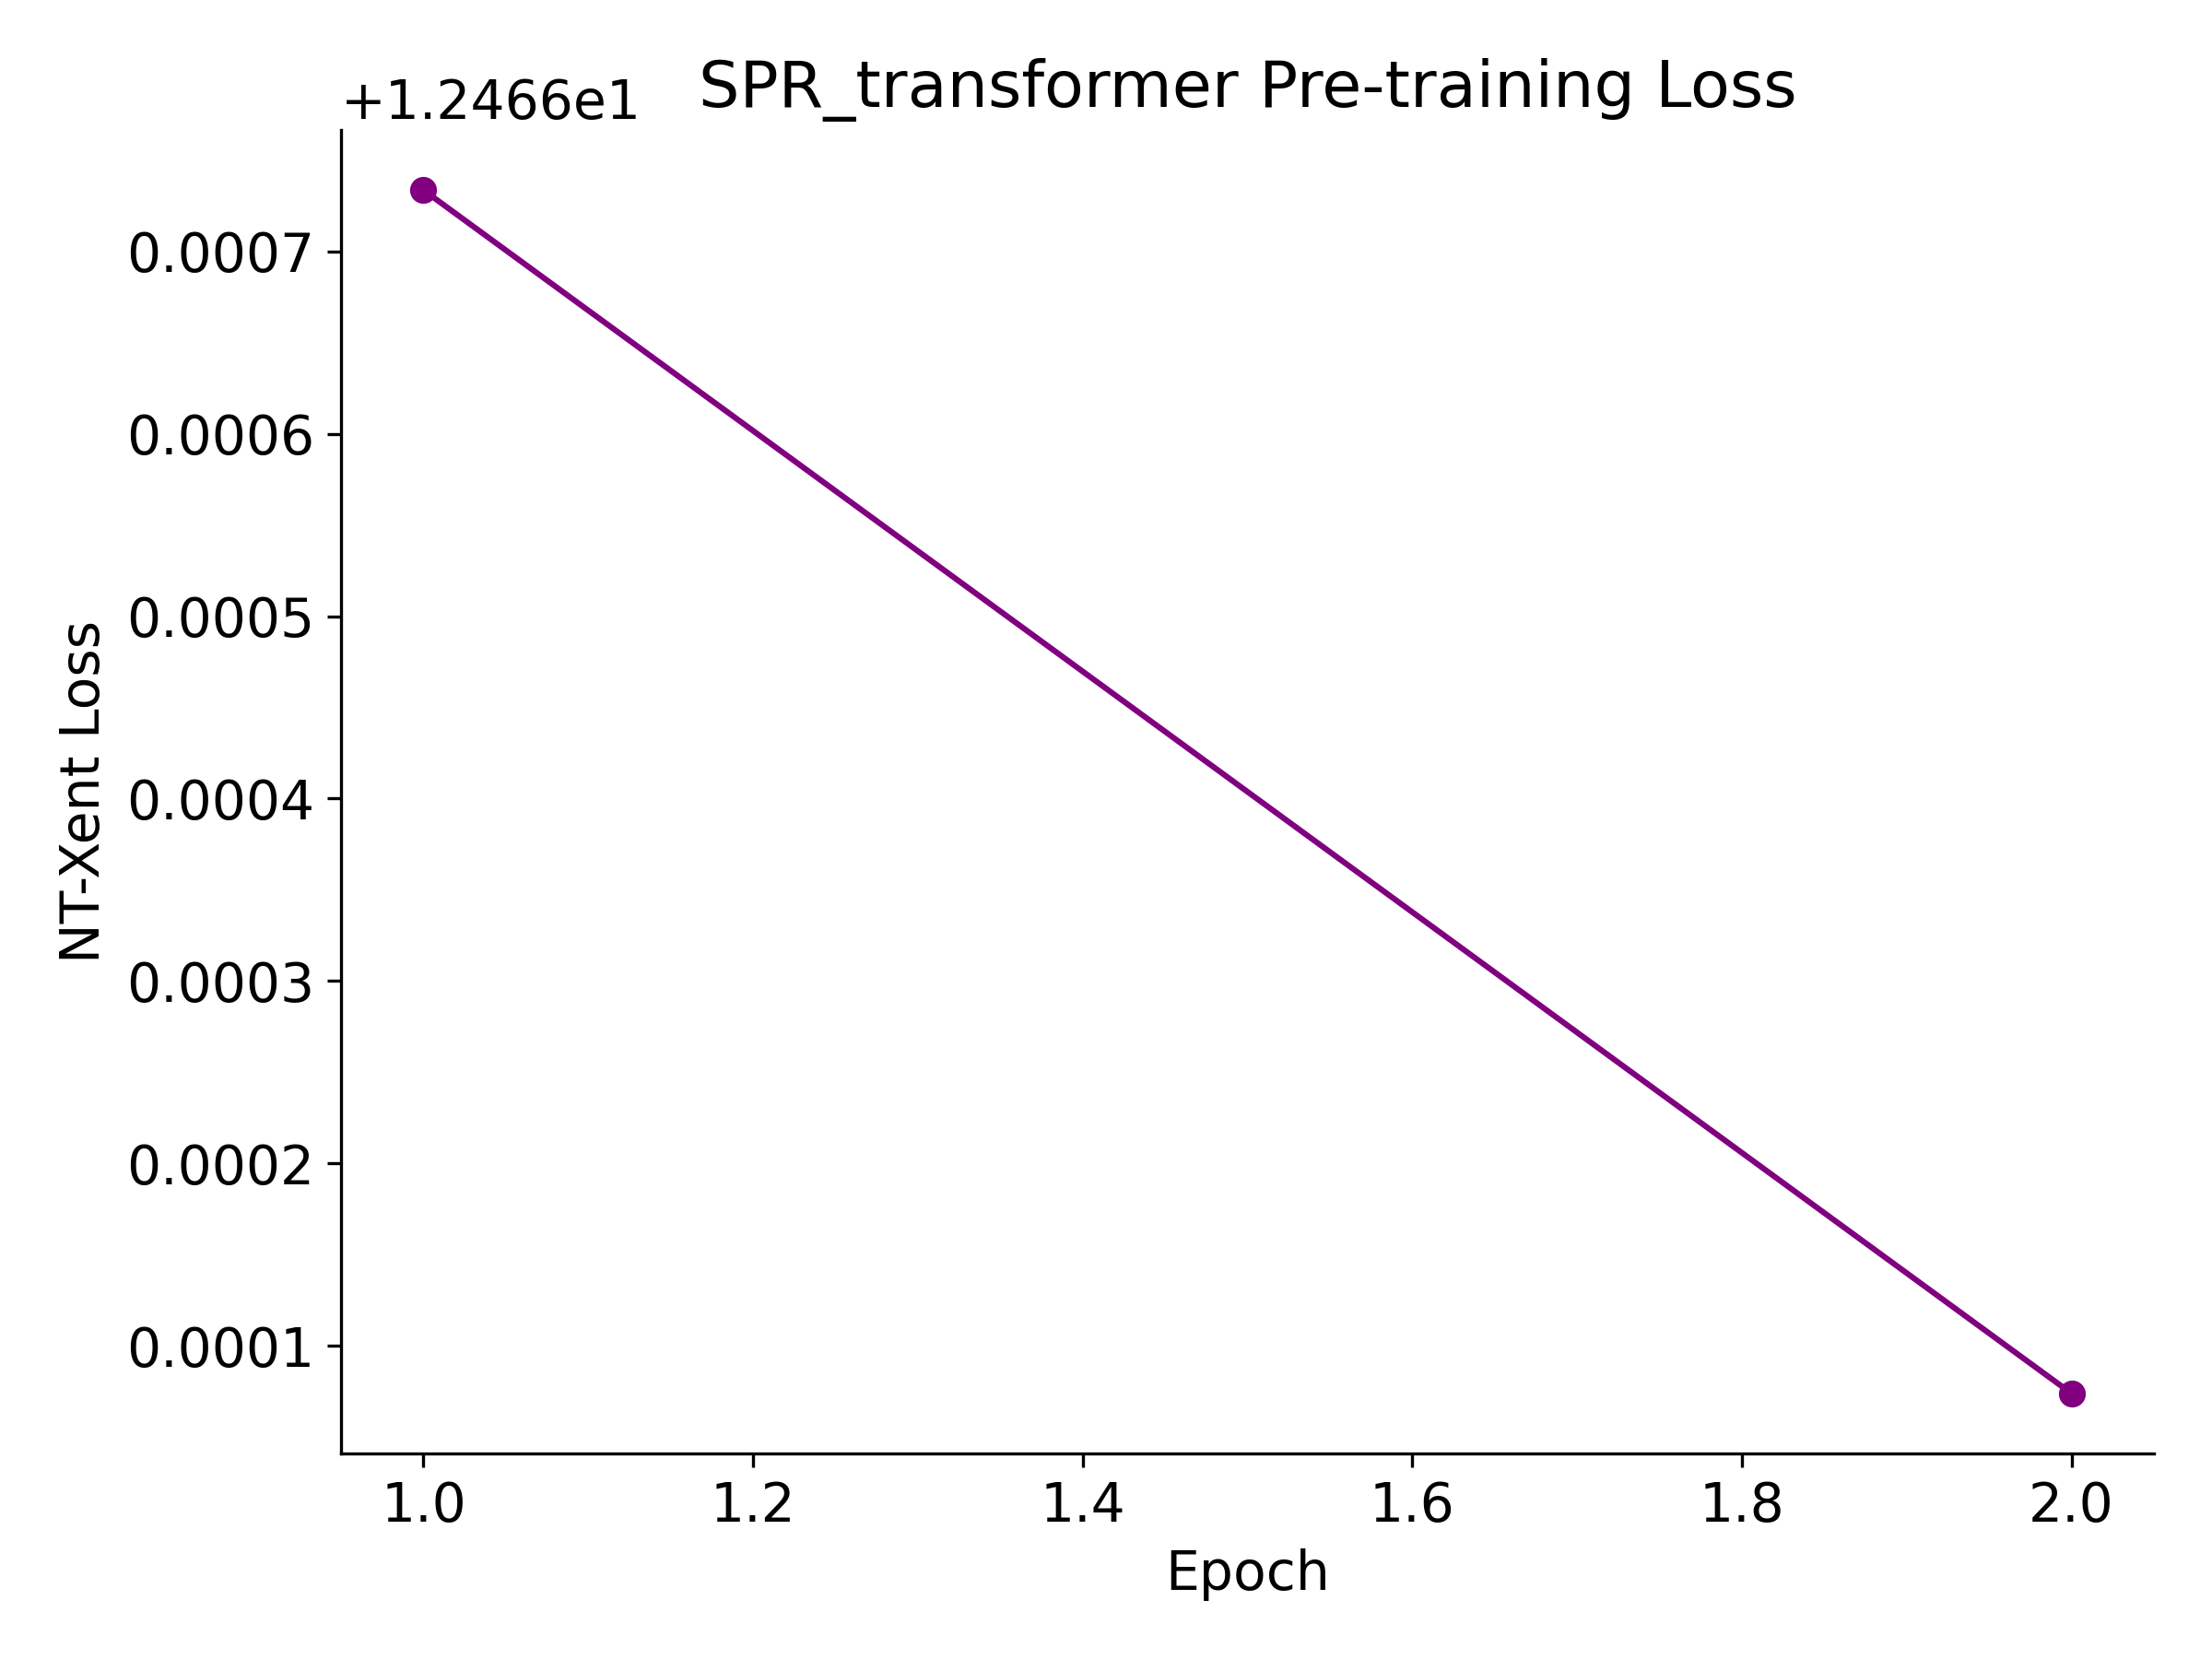
\includegraphics[width=0.35\textwidth]{research_pretrain_loss.png}
\caption{Pre-training loss under research settings.}
\label{fig:research_pretrain_loss}
\end{figure}

\end{document}